\clearpage
\subsubsection{Deltaic}
\begin{table}[h!]
\centering
\caption{Categorised GPR profile keywords for igneous environments. Geometry, reflectivity and continuity are shown in separate columns.}
\begin{tabular}{|p{6.5cm}|p{6.5cm}|}
\hline
\textbf{Geometry / Structure} & \textbf{Continuity / Amplitude / Reflectivity} \\
\hline
Parallel & High amplitude \\
Concave & Semi-continuous \\
Tangential & Discontinuous \\
Cross-bedding & Varied amplitude \\
Complex & High reflectivity \\
Subparallel & Low reflectivity \\
Multidirectional dipping & Varied reflectivity \\
Subhorizontal/Semi-horizontal & Low attenuation \\
Horizontal & High attenuation \\
Prograding & Continuous \\
Clinoform & Medium amplitude \\
Sigmoidal & Low amplitude \\
Dipping/Inclined/slight dipping & \\
Tabular & \\
Ridge & \\
Onlap & \\
Truncation & \\
Bounding surface & \\
Hyperbolic & \\
Convex/Curved& \\
Erosion / Erosional & \\
Hummocky/Sinuous & \\
Oblique & \\
Wedge & \\
Lenticular & \\
Chaotic & \\
Unconformity & \\
Undulating & \\
Toplap & \\
Semi-parallel & \\
\hline
\end{tabular}
\label{tab:coastal-keywords}
\end{table}
 
\begin{figure}[h!]
    \centering
    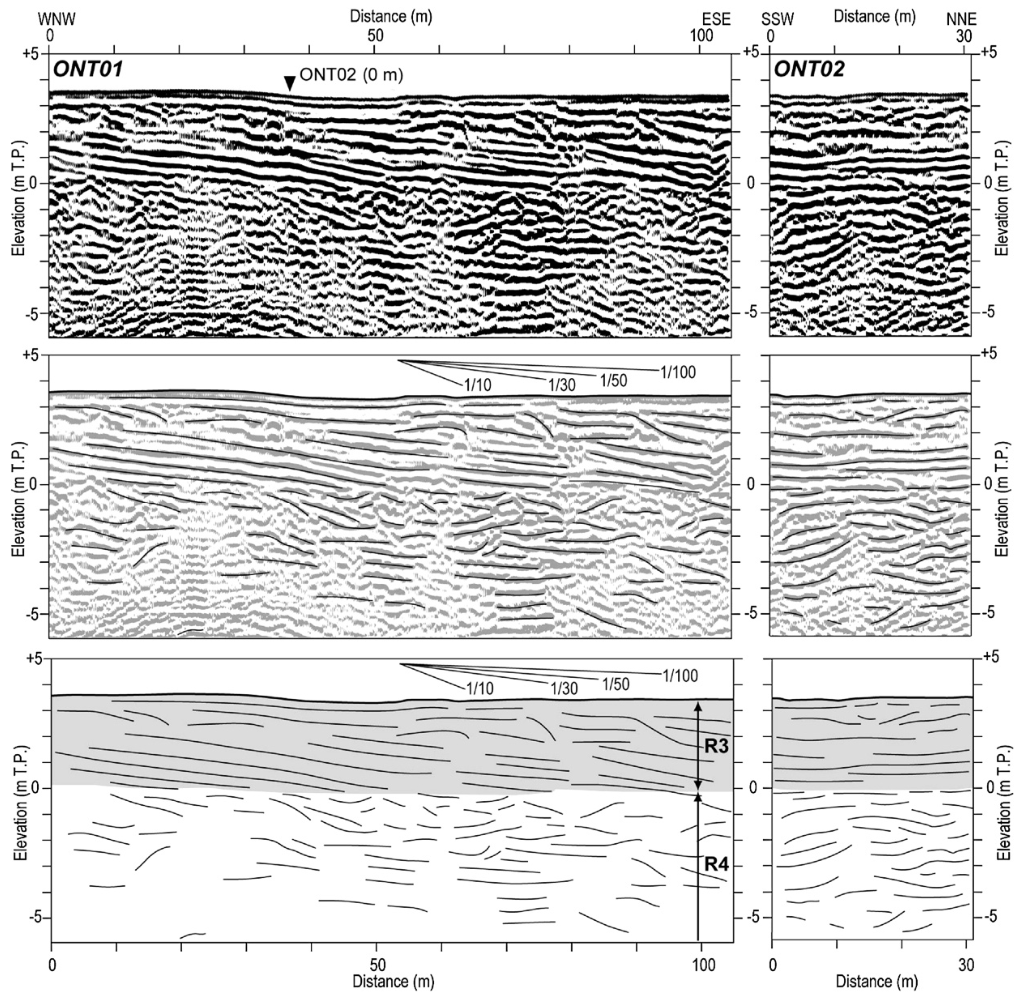
\includegraphics[width=0.9\linewidth]{Figures/0.2GPR/Tamura2008_2.png}
    \caption[Foreshore and upper shoreface deposits.]{Foreshore and upper shoreface deposits. \textbf{Keywords: } Parallel, concave, tangential, cross-bedding, complex, discontinuous, subparallel, low amplitude, multidirectional dipping  \citep{Tamura2008}.}
    \label{fig:Tamura2008-2}
\end{figure}

\begin{figure}[h!]
    \centering
    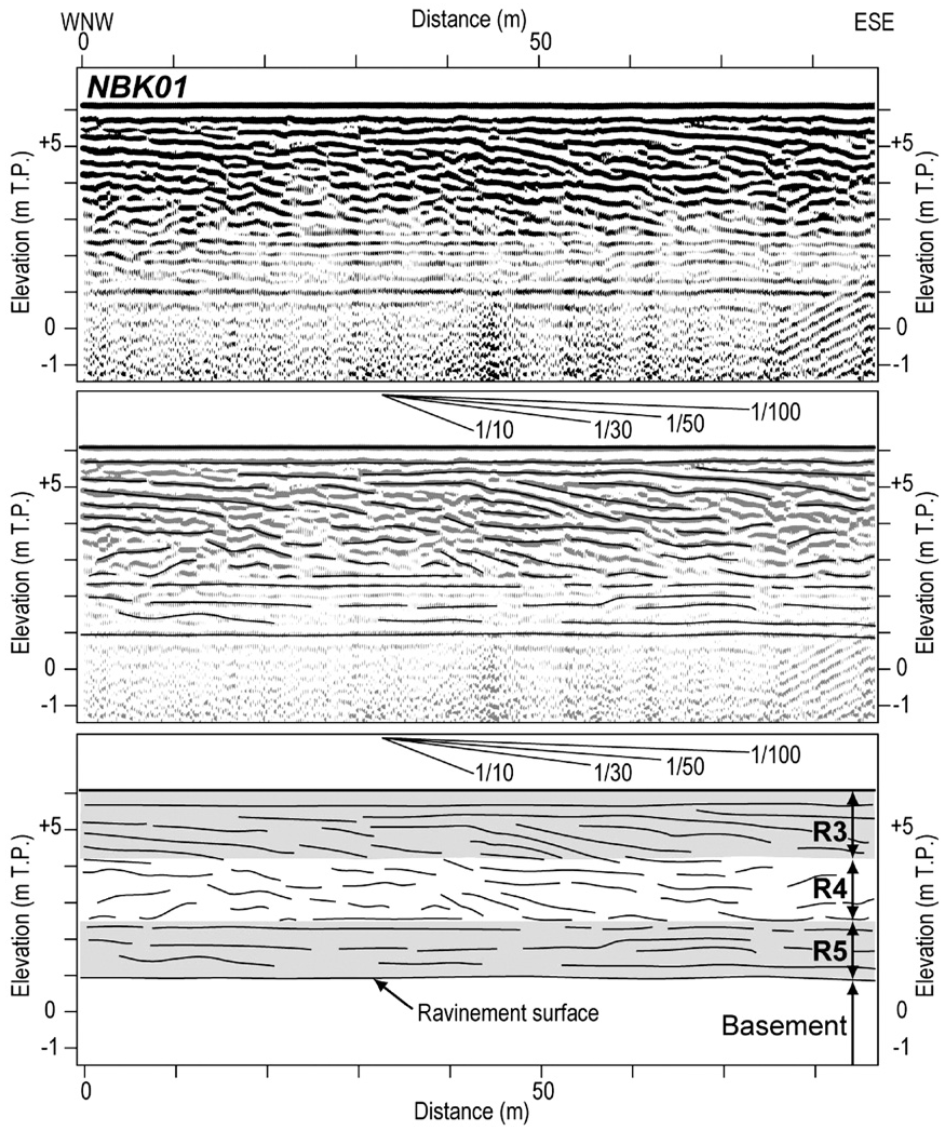
\includegraphics[width=0.9\linewidth]{Figures/0.2GPR/Tamura2008_4.png}
    \caption[Shore-normal transect (2).]{Shore-normal transect. \textbf{Keywords: } Continuous, subhorizontal, horizontal, discontinuous, multidirectional dipping, varied amplitude  \citep{Tamura2008}.}
    \label{fig:Tamura2008-4}
\end{figure}
\begin{landscape}
    \begin{figure}[h!]
    \centering
    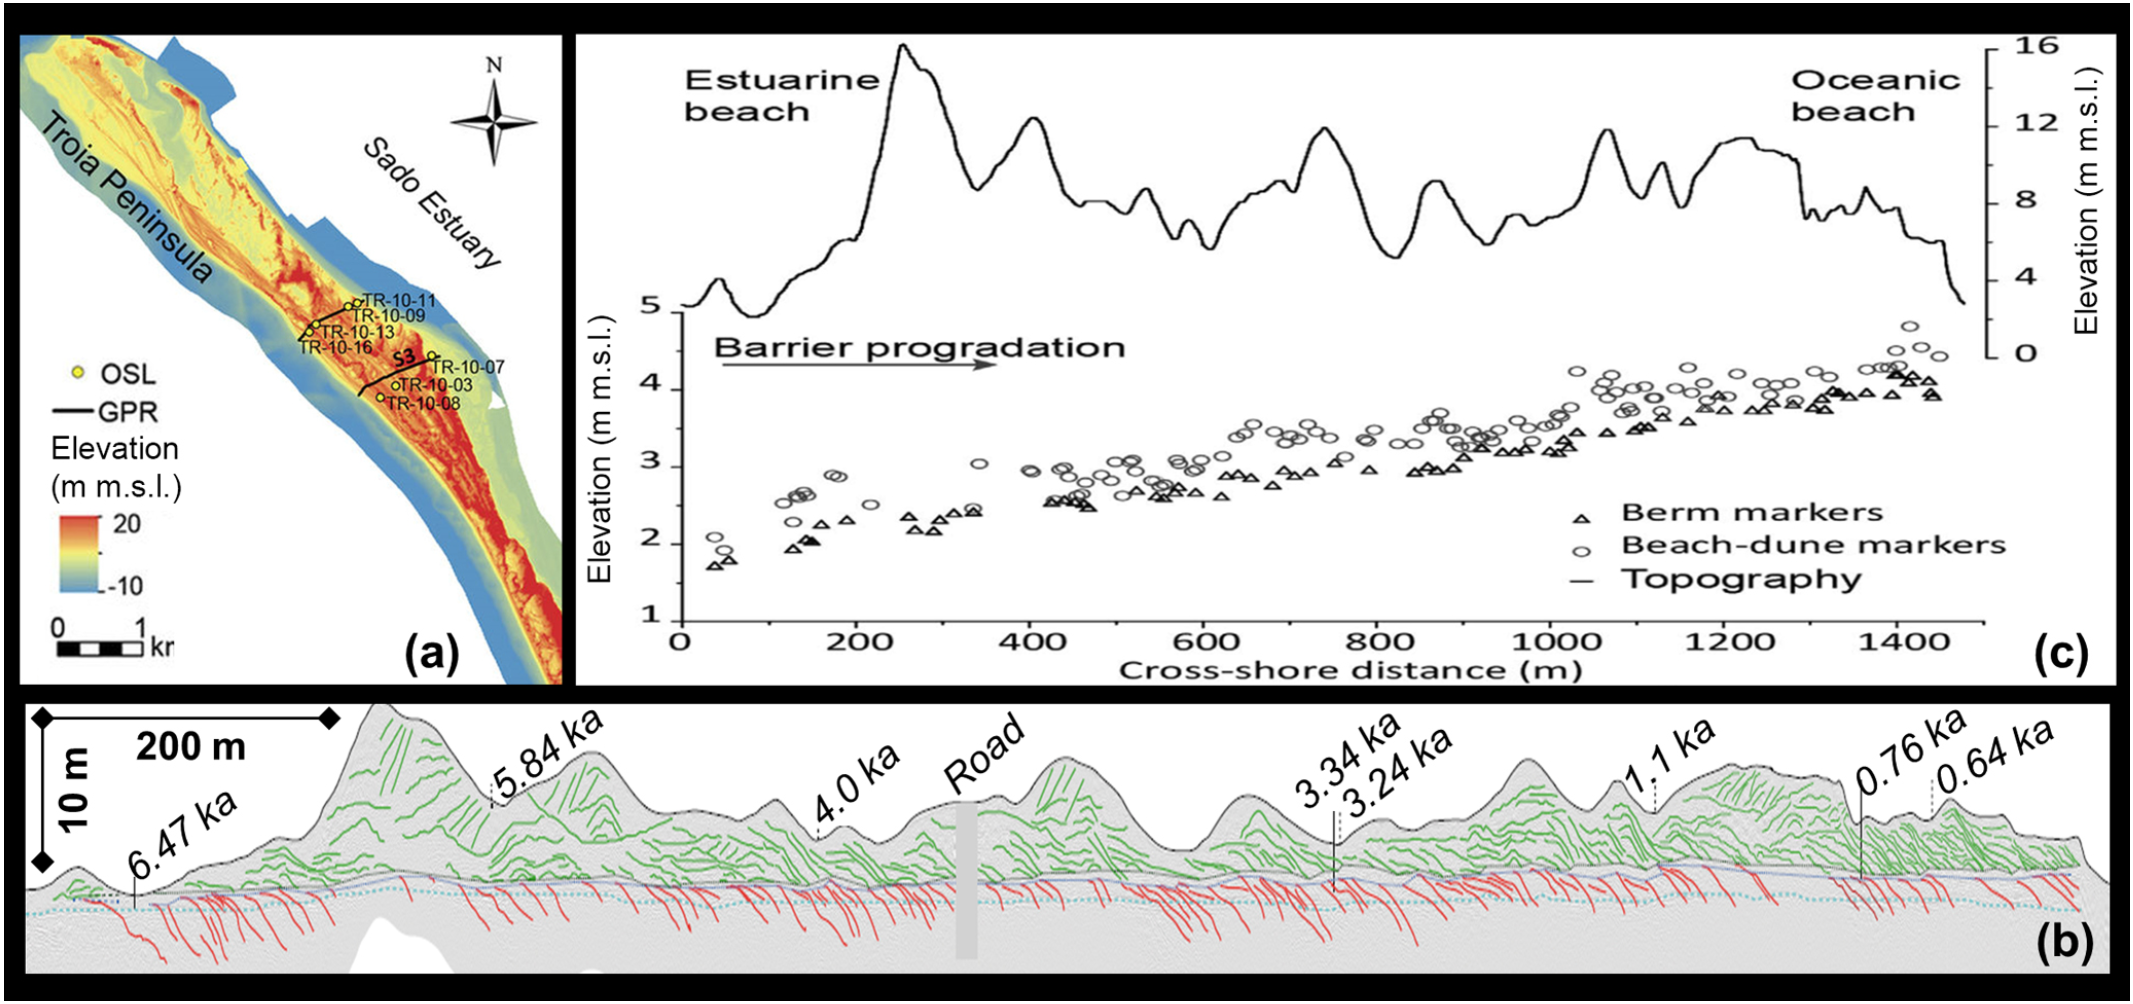
\includegraphics[width=0.9\linewidth]{Figures/0.2GPR/dougherty2019-1.png}
    \caption[Shoreline evolution (1).]{Shoreline evolution (1). \textbf{Keywords: } Prograding, clinoforms, sigmoidal, dipping, tabular, sub-horizontal, concave, downlap, ridge, continuous, semi-continuous, laterally extensive, varied amplitude, truncation, onlap \citep{Dougherty2019}.}
    \label{fig:dougherty2019-1}
\end{figure}
\end{landscape}

\begin{figure}[h!]
    \centering
    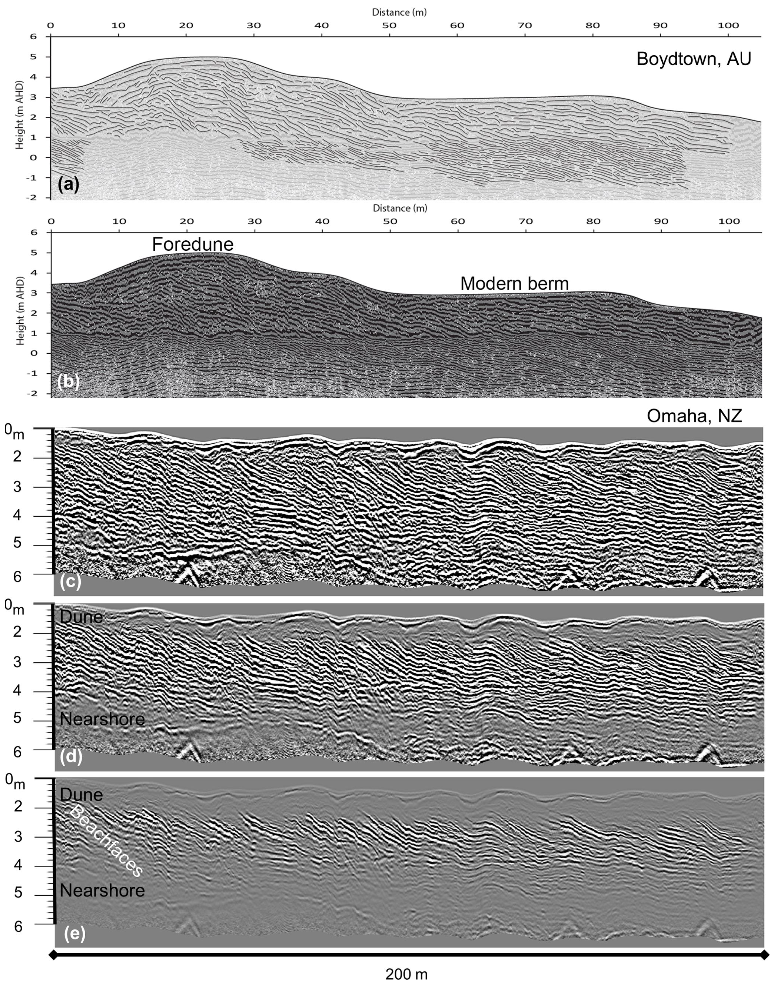
\includegraphics[width=0.9\linewidth]{Figures/0.2GPR/dougherty2019-2.png}
    \caption[Shoreline evolution (2).]{Shoreline evolution (2). \textbf{Keywords: } Prograding, clinoforms, sigmoidal, dipping, tabular, sub-horizontal, concave, downlap, ridge, continuous, semi-continuous, laterally extensive, varied amplitude, truncation, onlap \citep{Dougherty2019}.}
    \label{fig:dougherty2019-2}
\end{figure}

\begin{figure}[h!]
    \centering
    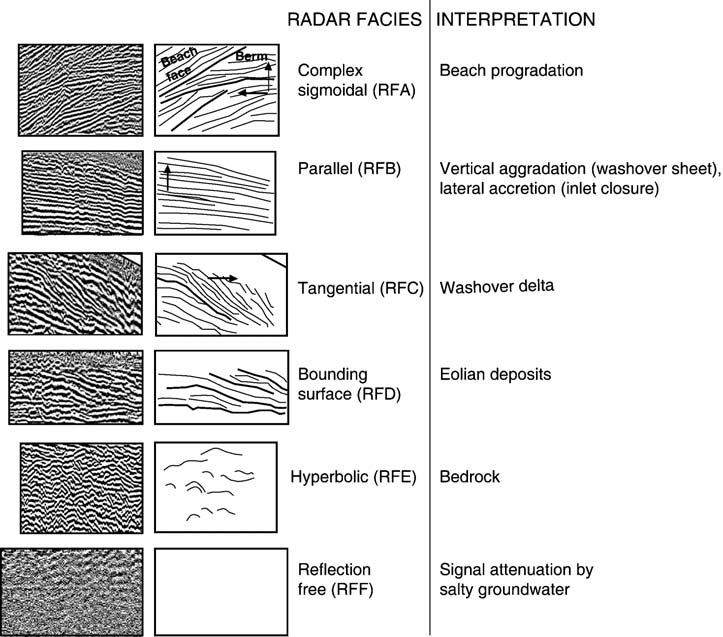
\includegraphics[width=0.9\linewidth]{Figures/0.2GPR/Costas2006_trace_1.png}
    \caption[Transgressive sand barrier (1).]{Transgressive sand barrier (1).\textbf{Keywords: } Sigmoidal, parallel, tangential, bounding surface, hyperbolic, dipping, high attenuation, low reflectivity, high reflectivity \citep{Costas2006}.}
    \label{fig:Costas2006-1}
\end{figure}

\begin{landscape}
\begin{figure}[h!]
    \centering
    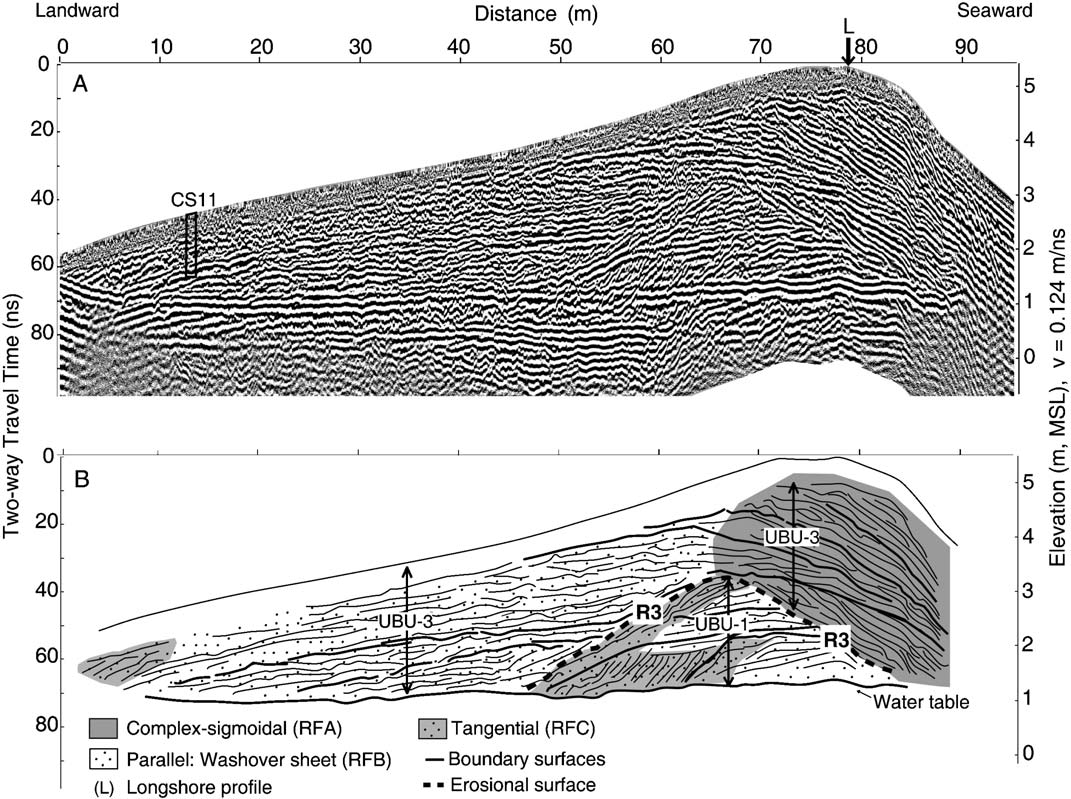
\includegraphics[width=0.8\linewidth]{Figures/0.2GPR/Costas2006_trace_2.png}
    \caption[Transgressive sand barrier (2).]{Transgressive sand barrier (2). \textbf{Keywords: } Parallel, tangential, multidirectional dipping, horizontal, erosion, high reflectivity, low attenuation, bounding surface, sigmoidal, semi-continuous, discontinuous \citep{Costas2006}.}
    \label{fig:Costas2006-2}
\end{figure}
\end{landscape}

\begin{figure}[h!]
    \centering
    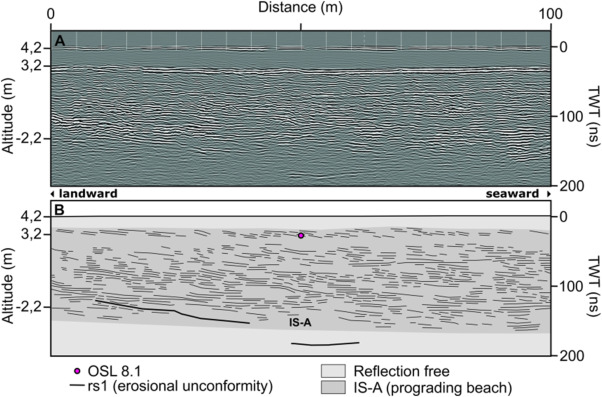
\includegraphics[width=0.8\linewidth]{Figures/0.2GPR/Figueiredo2021-gr4.jpg}
    \caption[Prograding beach ridge.]{Prograding beach ridge. \textbf{Keywords: } Prograding, clinoform, horizontal, dipping, tabular, semi-continuous, high reflectivity, medium reflectivity, high amplitude, moderate amplitude, downlap, onlap \citep{Figueiredo2021}.}
    \label{fig:Figueiredo2021-4}
\end{figure}

\begin{figure}[h!]
    \centering
    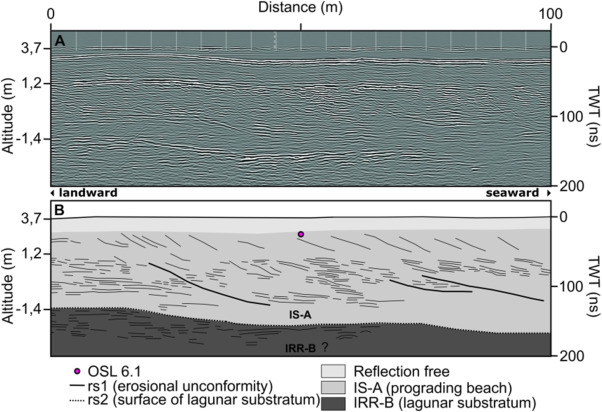
\includegraphics[width=0.8\linewidth]{Figures/0.2GPR/Figueiredo2021-gr5.jpg}
    \caption[Prograding beach ridge.]{Prograding beach ridge. \textbf{Keywords: } Sigmoidal, convex, continuous, medium reflectivity, high reflectivity, low amplitude, truncation, prograding, dipping \citep{Figueiredo2021}.}
    \label{fig:Figueiredo2021-5}
\end{figure}

\begin{landscape}
\begin{figure}[h!]
    \centering
    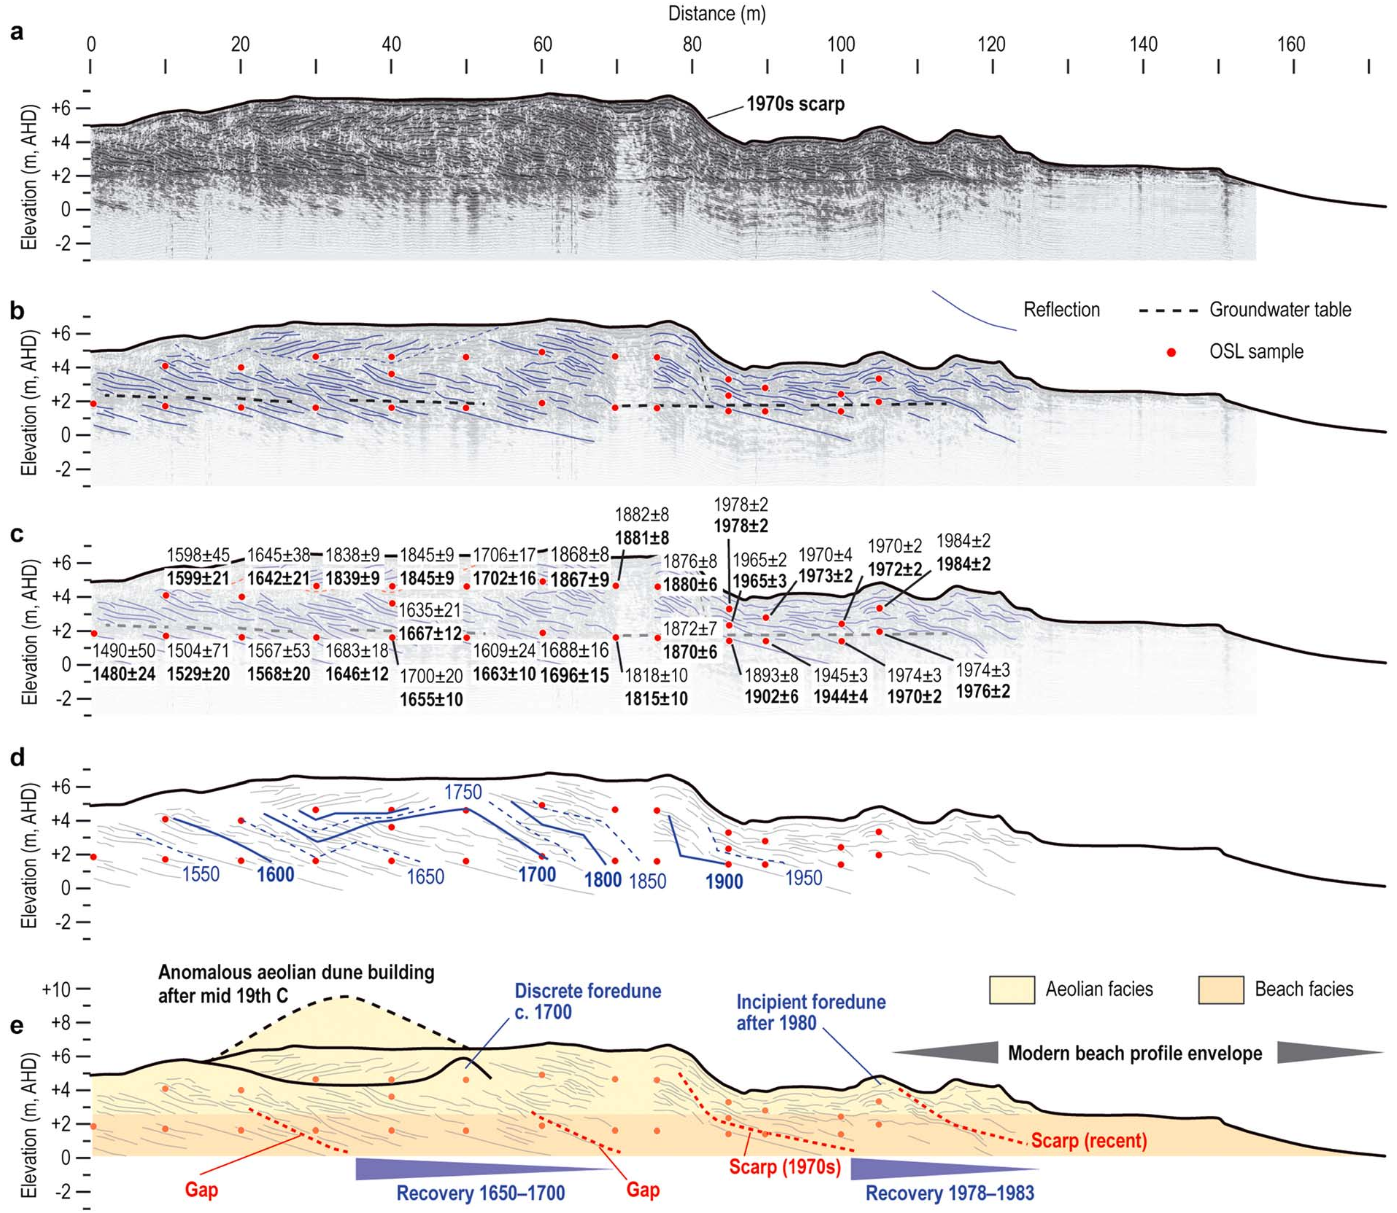
\includegraphics[width=0.75\linewidth]{Figures/0.2GPR/Tamura_2019_BR_Coast_er_1.png}
    \caption[Beach ridges and coastal erosion.]{Beach ridges and coastal erosion. \textbf{Keywords: } Dipping, continuous, semi-continuous, moderate amplitude, varied reflectivity, downlap, progradation, truncation, onlap, erosion \citep{Tamura2019}.}
    \label{fig:Tamura2019-1}
\end{figure}
\end{landscape}

\begin{landscape}
\begin{figure}[h!]
    \centering
    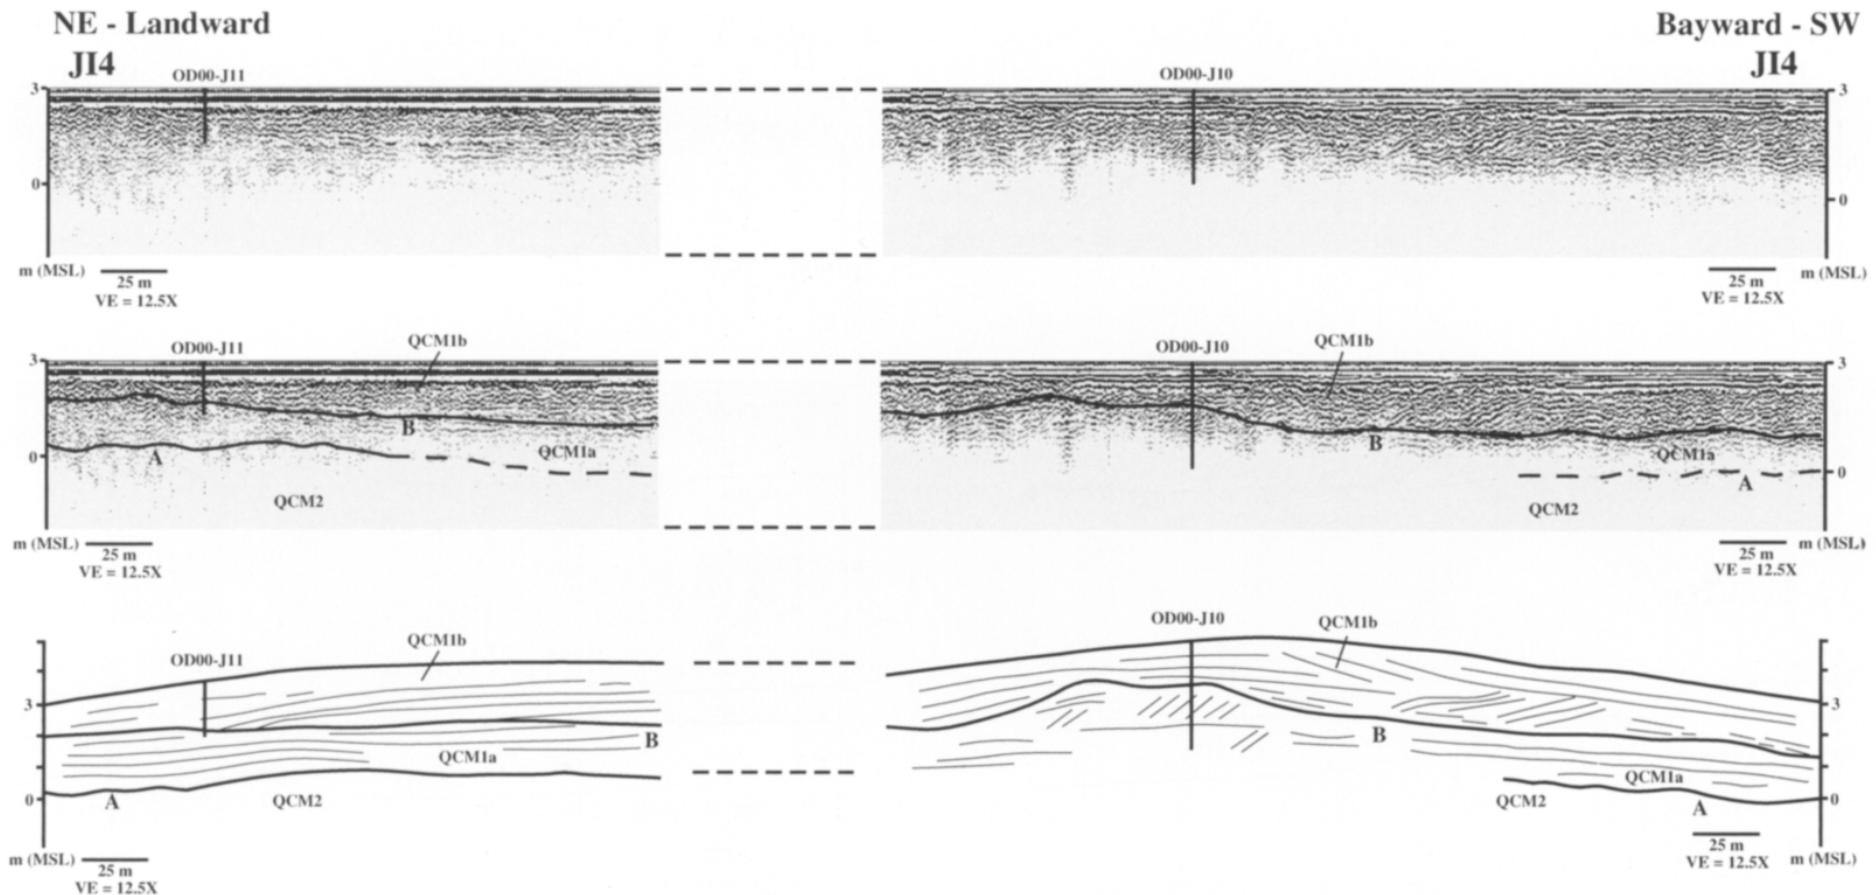
\includegraphics[width=0.9\linewidth]{Figures/0.2GPR/neal2003_1.png}
    \caption[Coarse-clastic beach-ridge deposits (1).]{Coarse-clastic beach-ridge deposits (1). \textbf{Keywords: } Dipping, tabular, semi-continuous, high amplitude, medium amplitude, truncation, downlap, prograding, onlap \citep{Neal2003}.}
    \label{fig:Neal2003-1}
\end{figure}
\end{landscape}

\begin{landscape}
  \begin{figure}[h!]
    \centering
    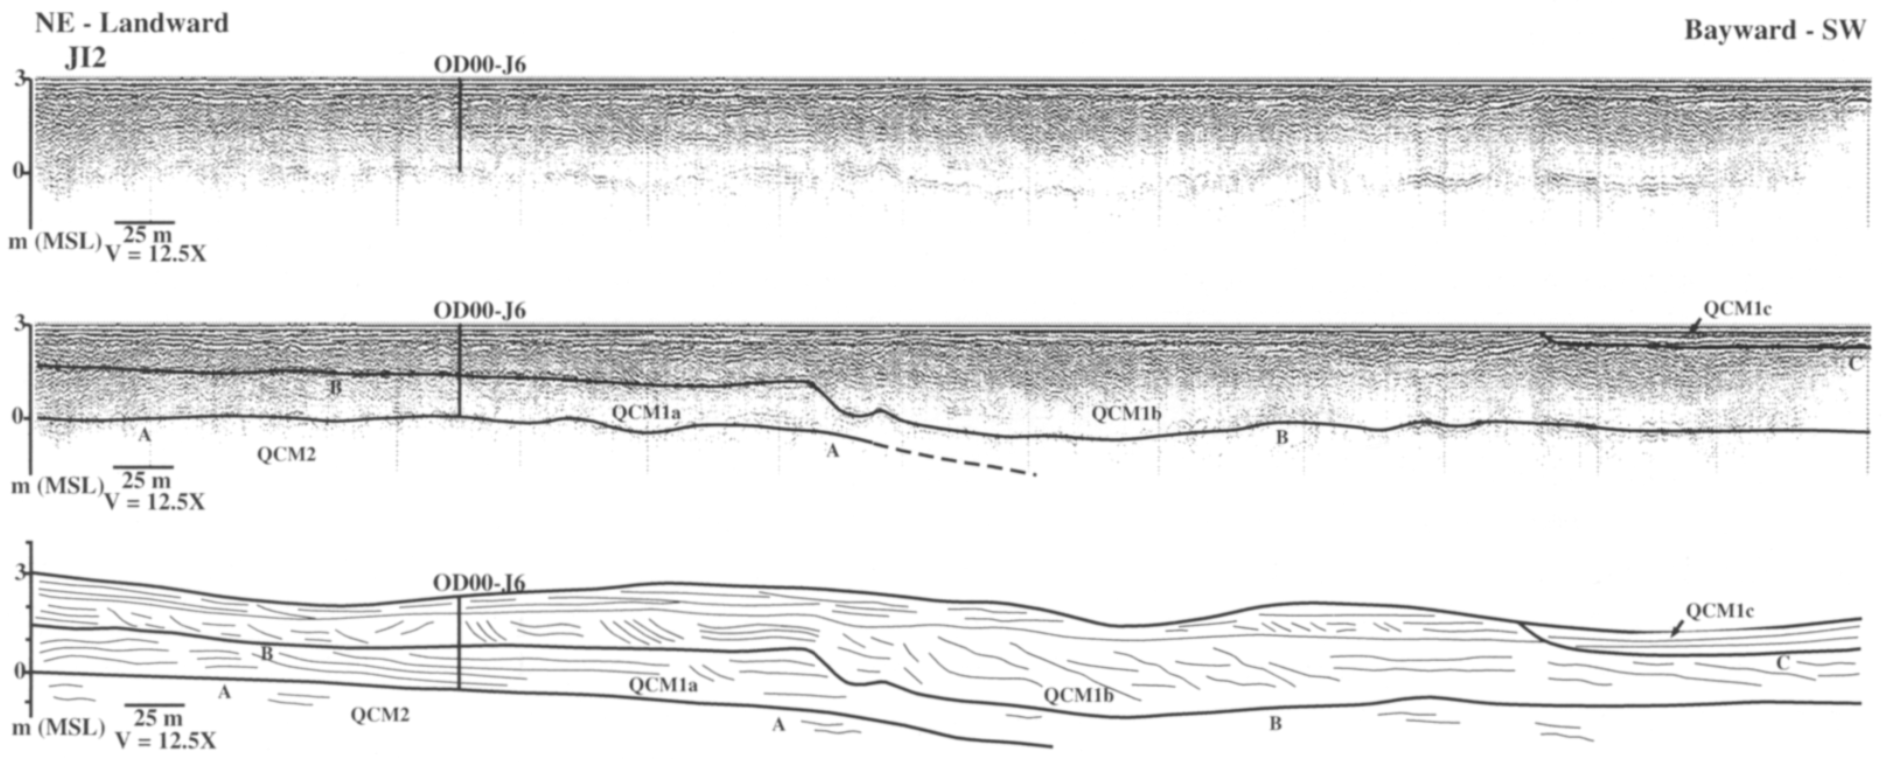
\includegraphics[width=0.9\linewidth]{Figures/0.2GPR/neal2003_2.png}
    \caption[Coarse-clastic beach-ridge deposits (2).]{Coarse-clastic beach-ridge deposits (2).\textbf{Keywords: } Sub-horizontal, lenticular, dipping, discontinuous, continuous, low amplitude, low reflectivity, high amplitude, erosion, bounding \citep{Neal2003}.}
    \label{fig:Neal2003-2}
\end{figure}  
\end{landscape}

\begin{figure}[h!]
    \centering
    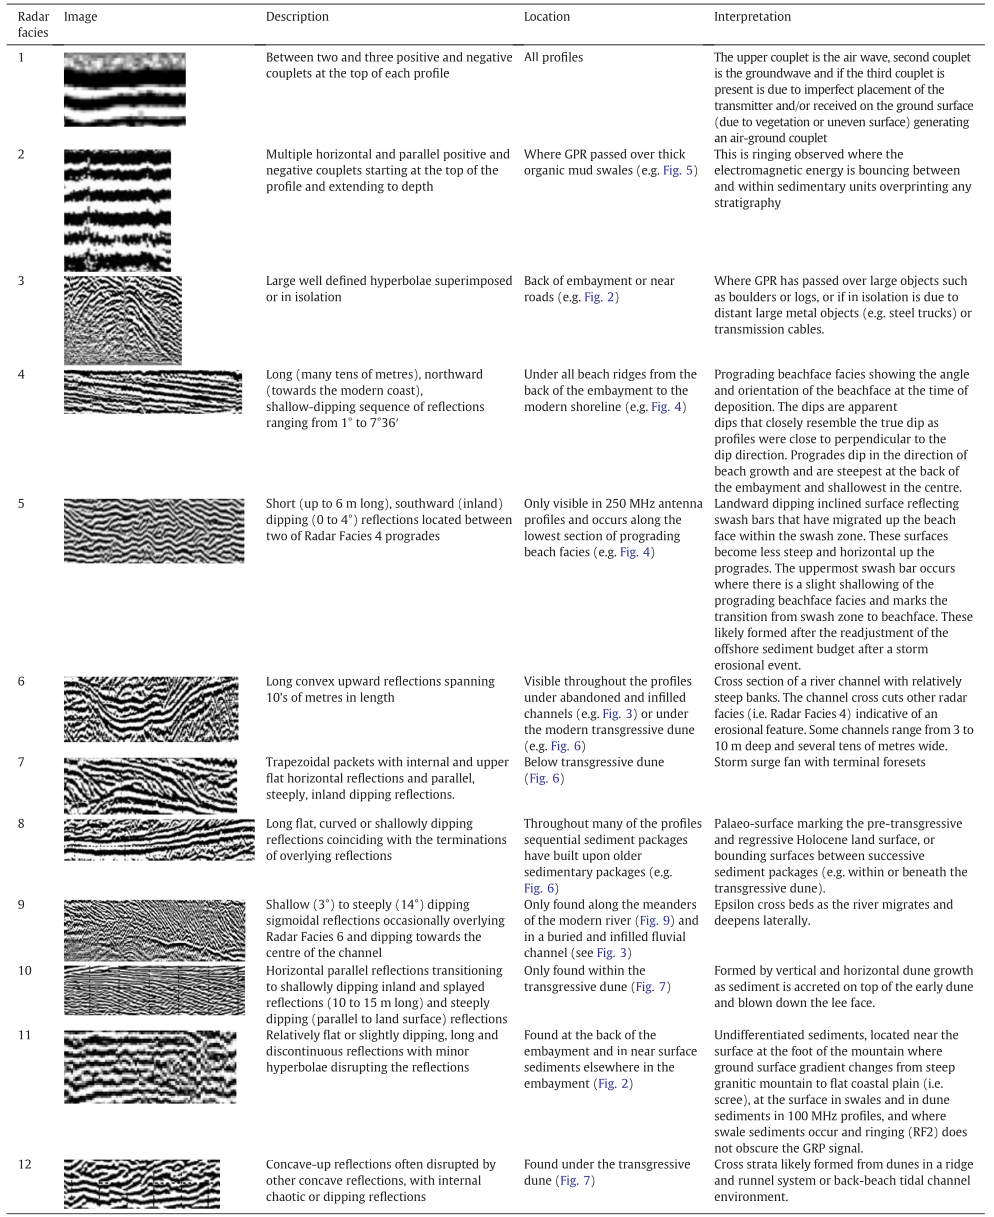
\includegraphics[width=0.9\linewidth]{Figures/0.2GPR/Gourmanis2020_coastal.png}
    \caption[Holocene evolution of coastal embayment.]{Holocene evolution of coastal embayment. \textbf{Keywords: } Horizontal, parallel, hyperbola, dipping, prograding, convex, horizontal, curved, sigmoidal, discontinuous, chaotic, semi-continuous, high reflectivity, low reflectivity \citep{Guramanis2020}.}
    \label{fig:Gourmanis2020-1}
\end{figure}

\begin{figure}[h!]
    \centering
    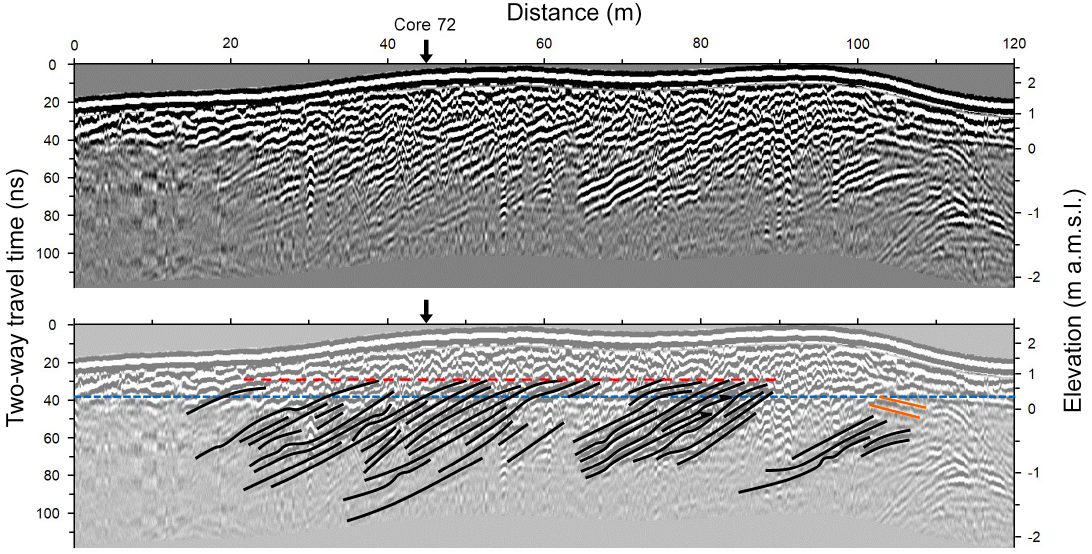
\includegraphics[width=0.9\linewidth]{Figures/0.2GPR/Nooren_2017_beach.png}
    \caption[Beach ridge plain.]{Beach ridge plain. \textbf{Keywords: } Dipping, parallel, erosion, semi-continuous, discontinuous, chaotic, high reflectivity, low reflectivity \citep{Nooren2017}.}
    \label{fig:Nooren2017-1}
\end{figure}

\begin{figure}[h!]
    \centering
    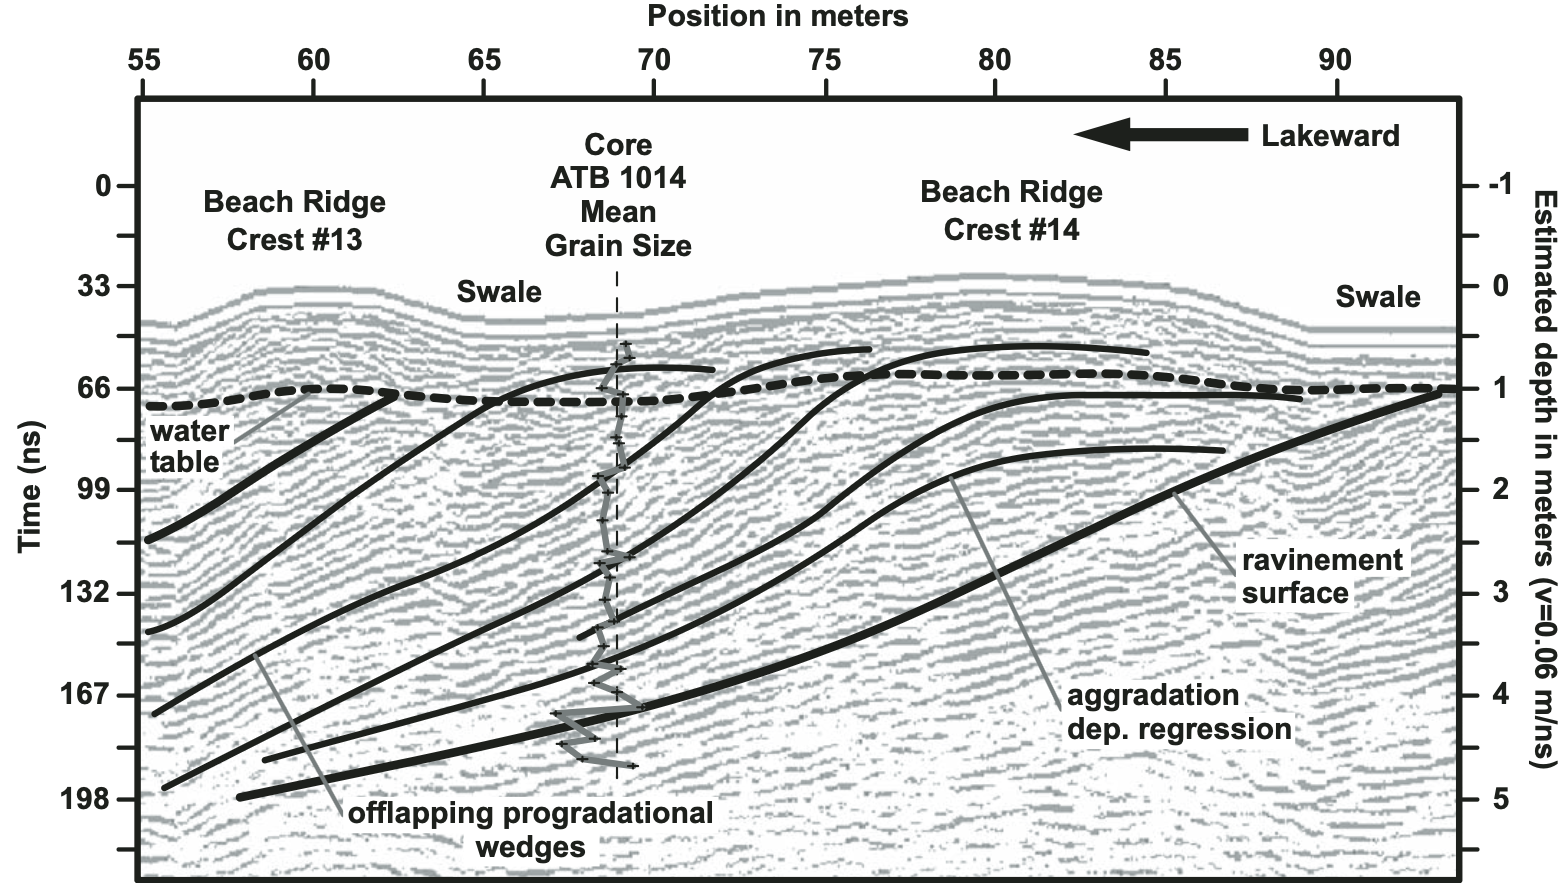
\includegraphics[width=0.9\linewidth]{Figures/0.2GPR/Johnston2007-2.png}
    \caption[Beach ridge development.]{Beach ridge development. \textbf{Keywords: } Dipping, continuous, discontinuous, parallel, hummocky, erosion, high reflectivity, low reflectivity \citep{Johnston2007}.}
\end{figure} 


\begin{figure}[h!]
    \centering
    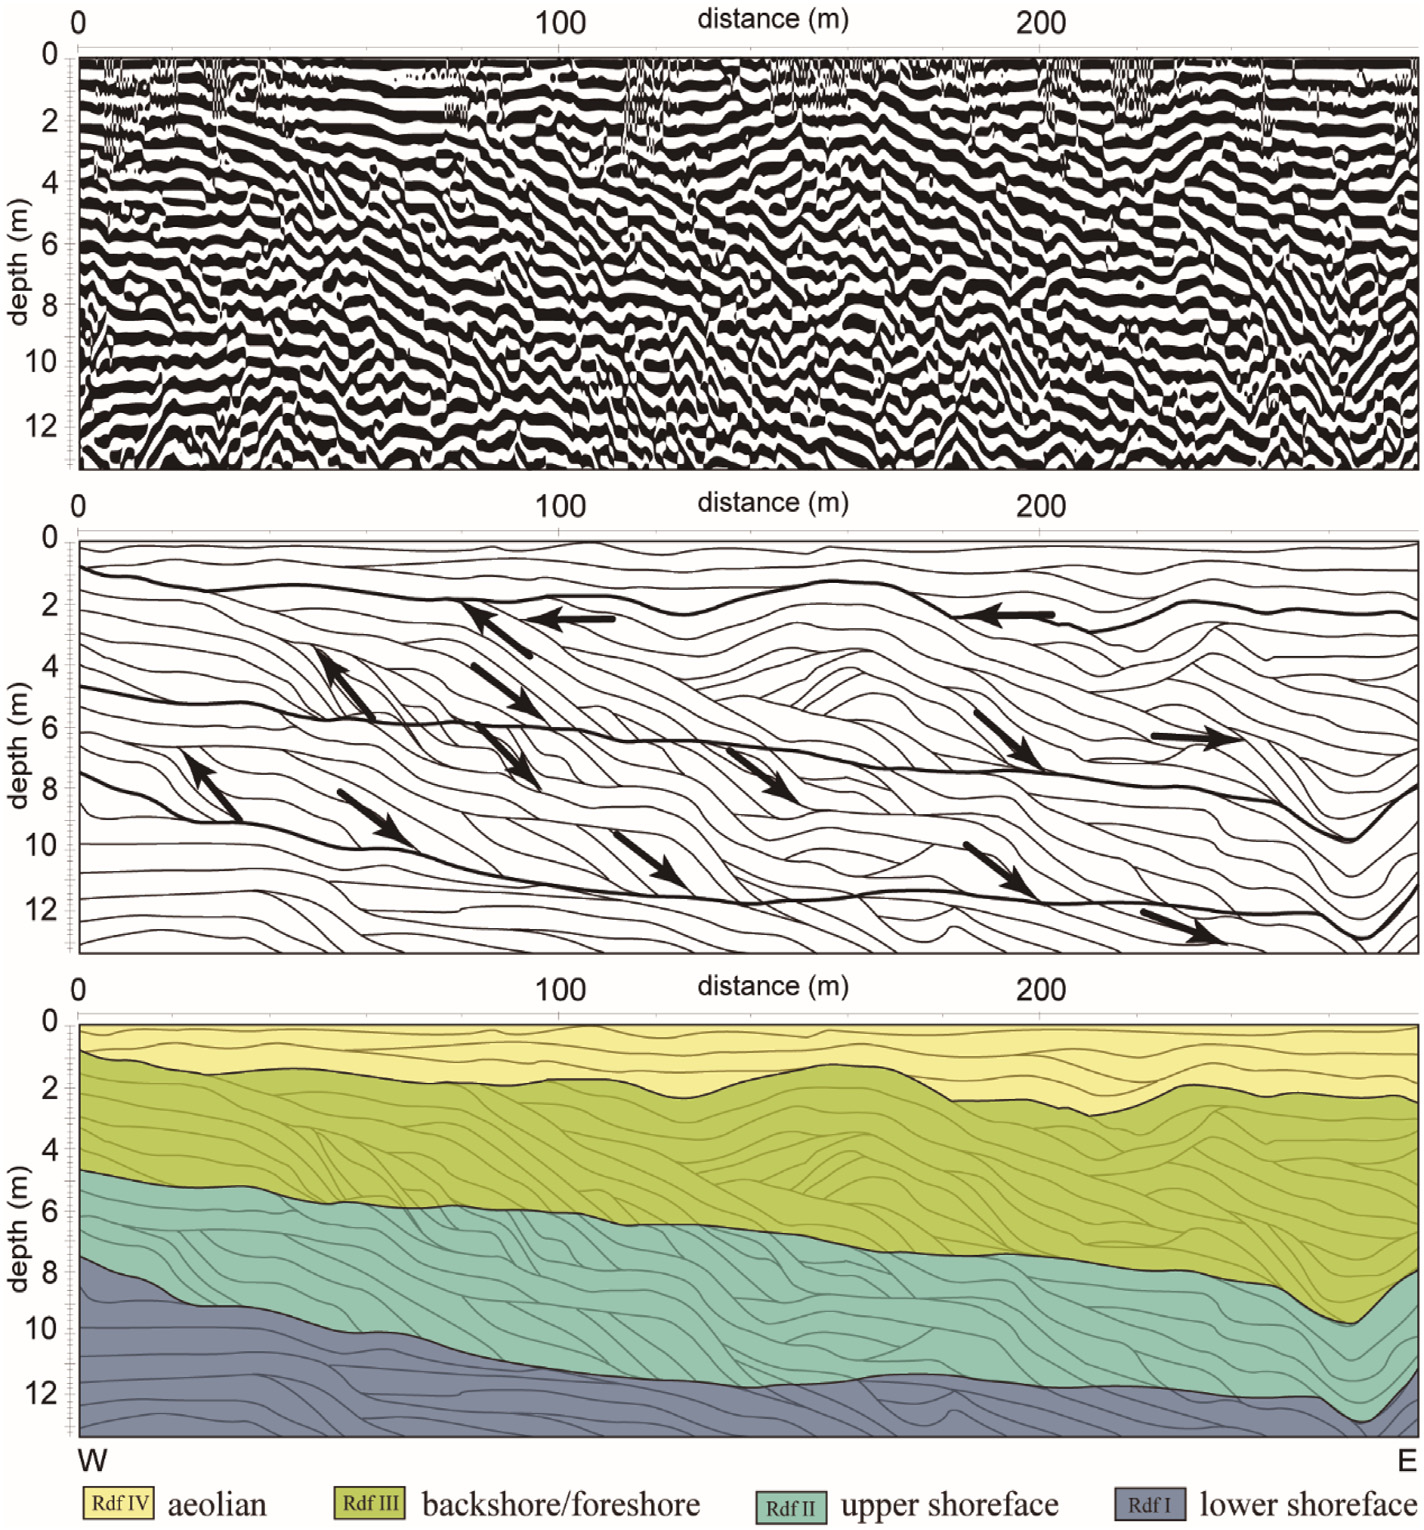
\includegraphics[width=0.9\linewidth]{Figures/0.2GPR/Leandro2018_coastal_2.png}
    \caption[Coastal depositional environments.]{Coastal depositional environments. \textbf{Keywords: } Erosional, dipping, chaotic, hummocky, onlap, downlap, truncation, high reflectivity, semi-horizontal, semi-parallel \citep{Leandro2019}.}
    \label{fig:Leandro2019-2}
\end{figure}

\begin{landscape}
    \begin{figure}[h!]
    \centering
    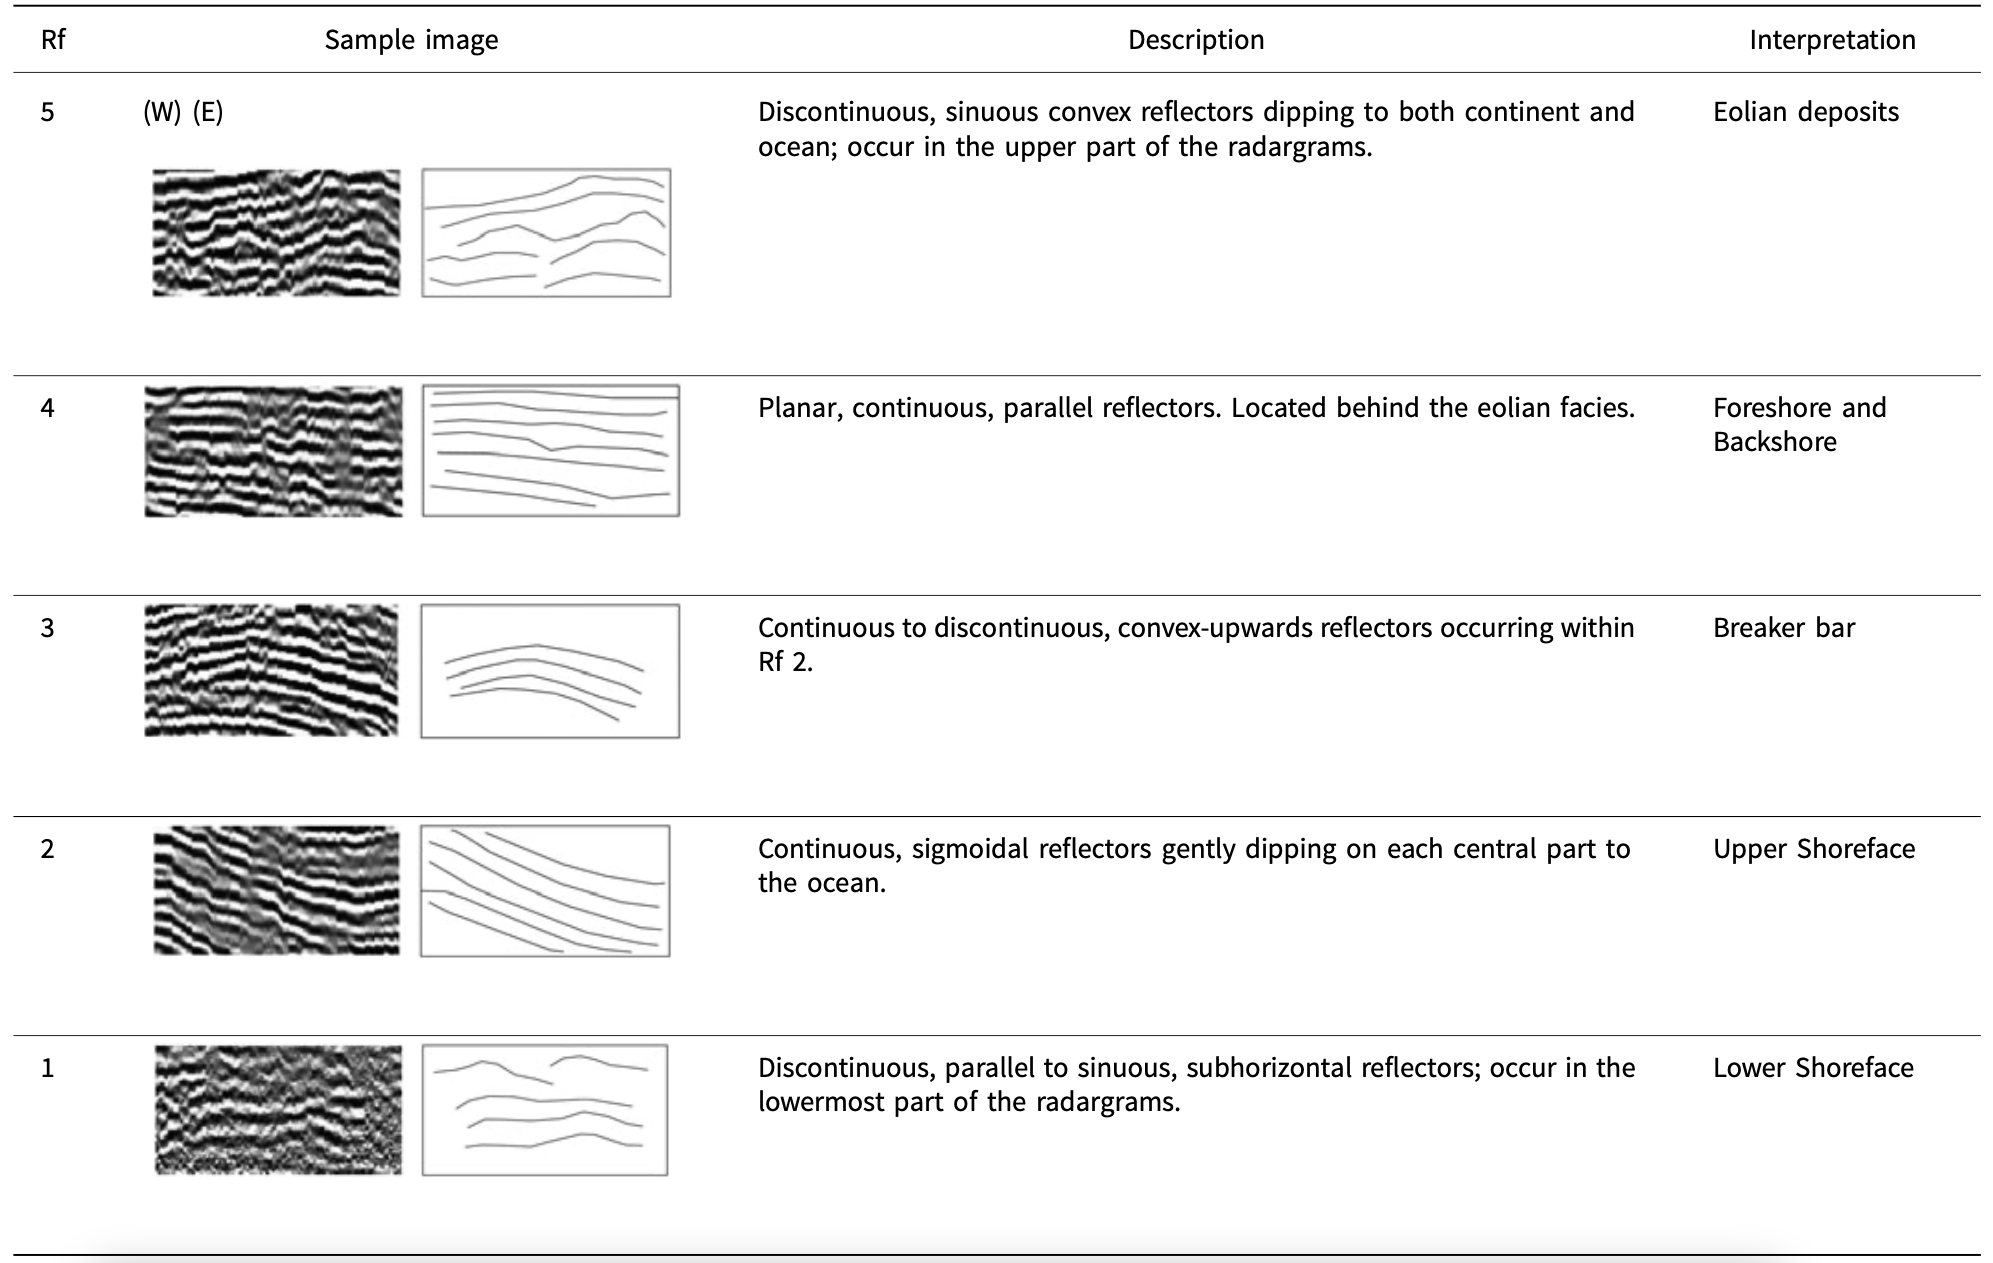
\includegraphics[width=0.9\linewidth]{Figures/0.2GPR/Santos2022_2.png}
    \caption[Micro-tidal barrier.]{Micro-tidal barrier. \textbf{Keywords: } Discontinuous, sinuous, convex, dipping, planar, continuous, sigmoidal, parallel, subhorizontal \citep{Santos2022}.}
    \label{fig:Santos2022-2}
\end{figure}
\end{landscape}

\begin{figure}[h!]
    \centering
    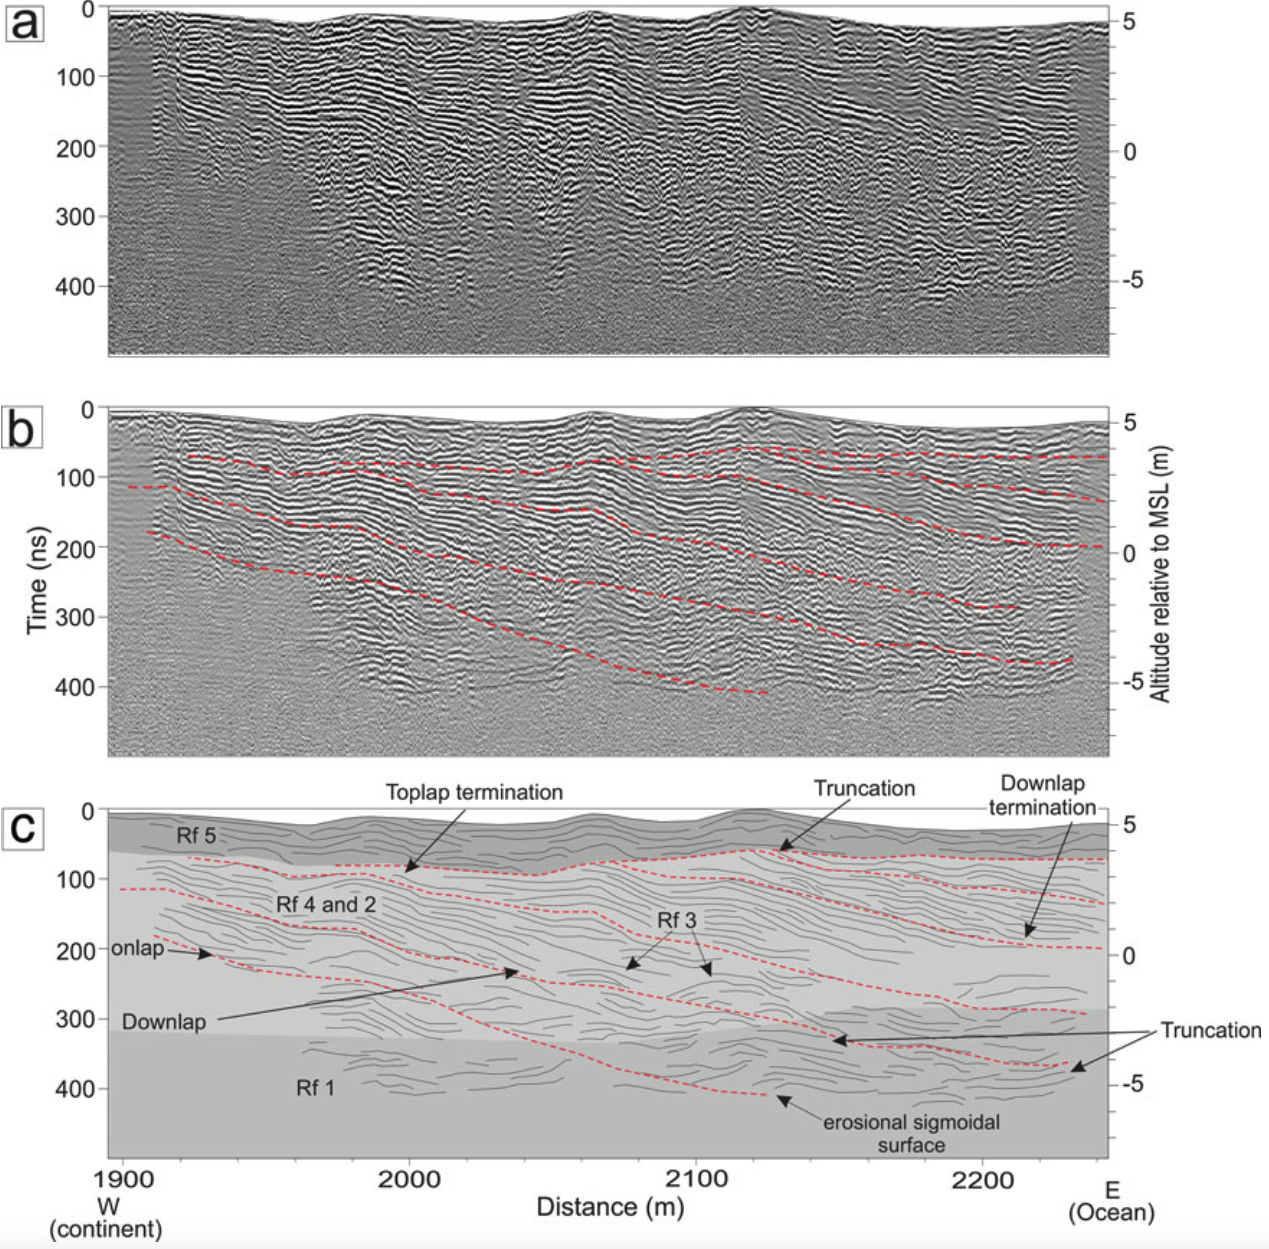
\includegraphics[width=0.9\linewidth]{Figures/0.2GPR/Santos2022_3.png}
    \caption[Micro-tidal barrier.]{Micro-tidal barrier. \textbf{Keywords: } Sigmoidal, truncation, downlap, toplap, and onlap \citep{Santos2022}.}
    \label{fig:Santos2022-3}
\end{figure}

\begin{landscape}
\begin{figure}[h!]
    \centering
    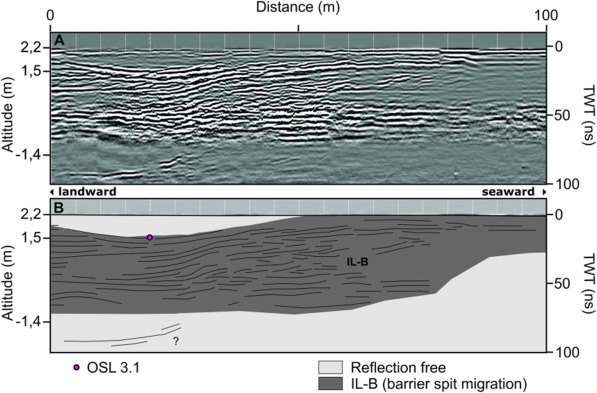
\includegraphics[width=0.9\linewidth]{Figures/0.2GPR/Figueiredo2021-gr8.jpg}
    \caption[Late Holocene evolution of sedimentary cape.]{Late Holocene evolution of sedimentary cape. \textbf{Keywords: } Discontinuous, varied reflectivity, semi-horizontal, chaotic, semi-parallel, slight dipping \citep{Figueiredo2021}.}
    \label{fig:Figueiredo2021-8}
\end{figure}
\end{landscape}
\clearpage

\begin{figure}[h!]
    \centering
    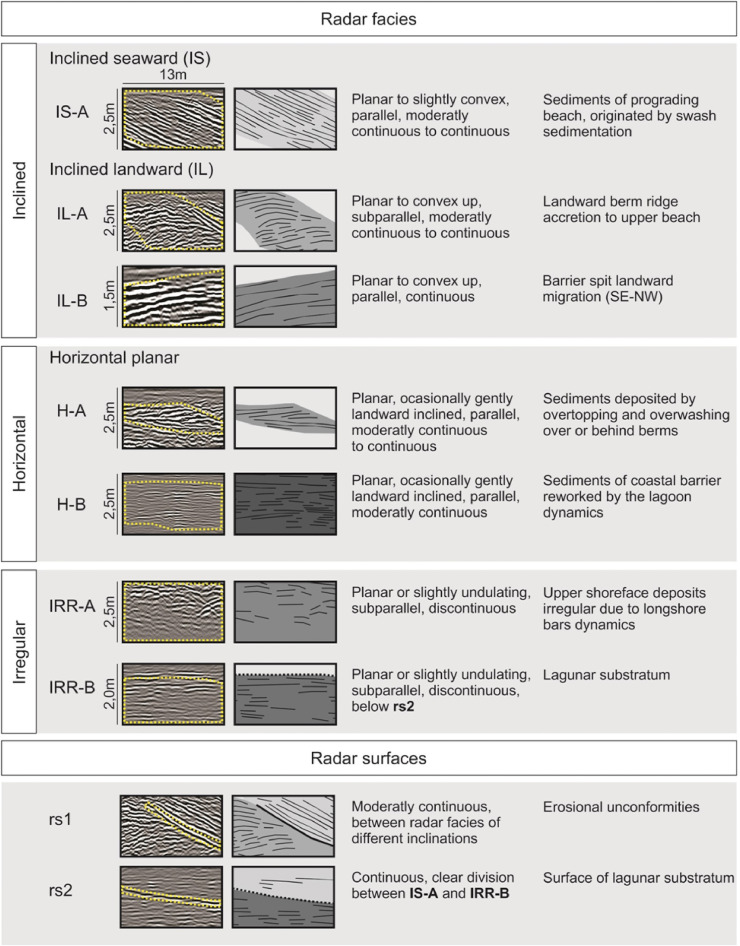
\includegraphics[width=0.9\linewidth]{Figures/0.2GPR/Figueiredo2021-fx1.jpg}
    \caption[Late Holocene evolution of sedimentary cape.]{Late Holocene evolution of sedimentary cape. \textbf{Keywords: } Inclined, horizontal, irregular, planar, convex, parallel, continuous, subparallel, undulating, discontinuous, unconformity, dipping \citep{Figueiredo2021}.}
    \label{fig:Figueiredo2021-1}
\end{figure}
\clearpage
